\section{Approach} 

There are a multitude of approaches one could take to calibrate cameras, and the choice of strategy significantly influences the complexity of the mathematical techniques required. The diversity in these approaches stems from the inherent complexity of cameras and the need for adaptable methods to address specific goals and constraints of each application. Notably, the accuracy of the calibration is significantly influenced by how the camera model is constructed, as well as the type of calibration used \footcite{weisunRequirementsCamera2005}.

\subsection{Camera Model} \label{sec:camera_model}

A camera model is a projection model which approximates the function of a camera by describing a mathematical relationship between points in 3D space and its projection onto the sensor grid of the camera. In order to construct such a model, we must first understand the general workings of a camera.

The modern lens camera is highly sophisticated, built with an array of complex mechanisms and a wide range of features such as zoom and autofocus. However, we only need to focus on its three principal elements critical to image projection: the lens, the aperture, and the sensor grid (CCD). 

\begin{itemize}[leftmargin=!, itemindent=-5ex]
    \item \textbf{Lens} -- Focuses incoming light rays and projects it onto the sensor grid. Modern cameras have compound lenses (lenses made up of several lens elements) in order to minimize undesired effects such as aberration, blurriness, and distortion. 
    \item \textbf{Aperture} -- Controls the amount of light that reaches the sensor. By adjusting the aperture size, the exposure and depth of field can be modified.
    \item \textbf{Sensor Grid} -- Captures incoming light rays and converts this information into pixels on an image. 
\end{itemize}

\begin{figure}[H]
    \centering
    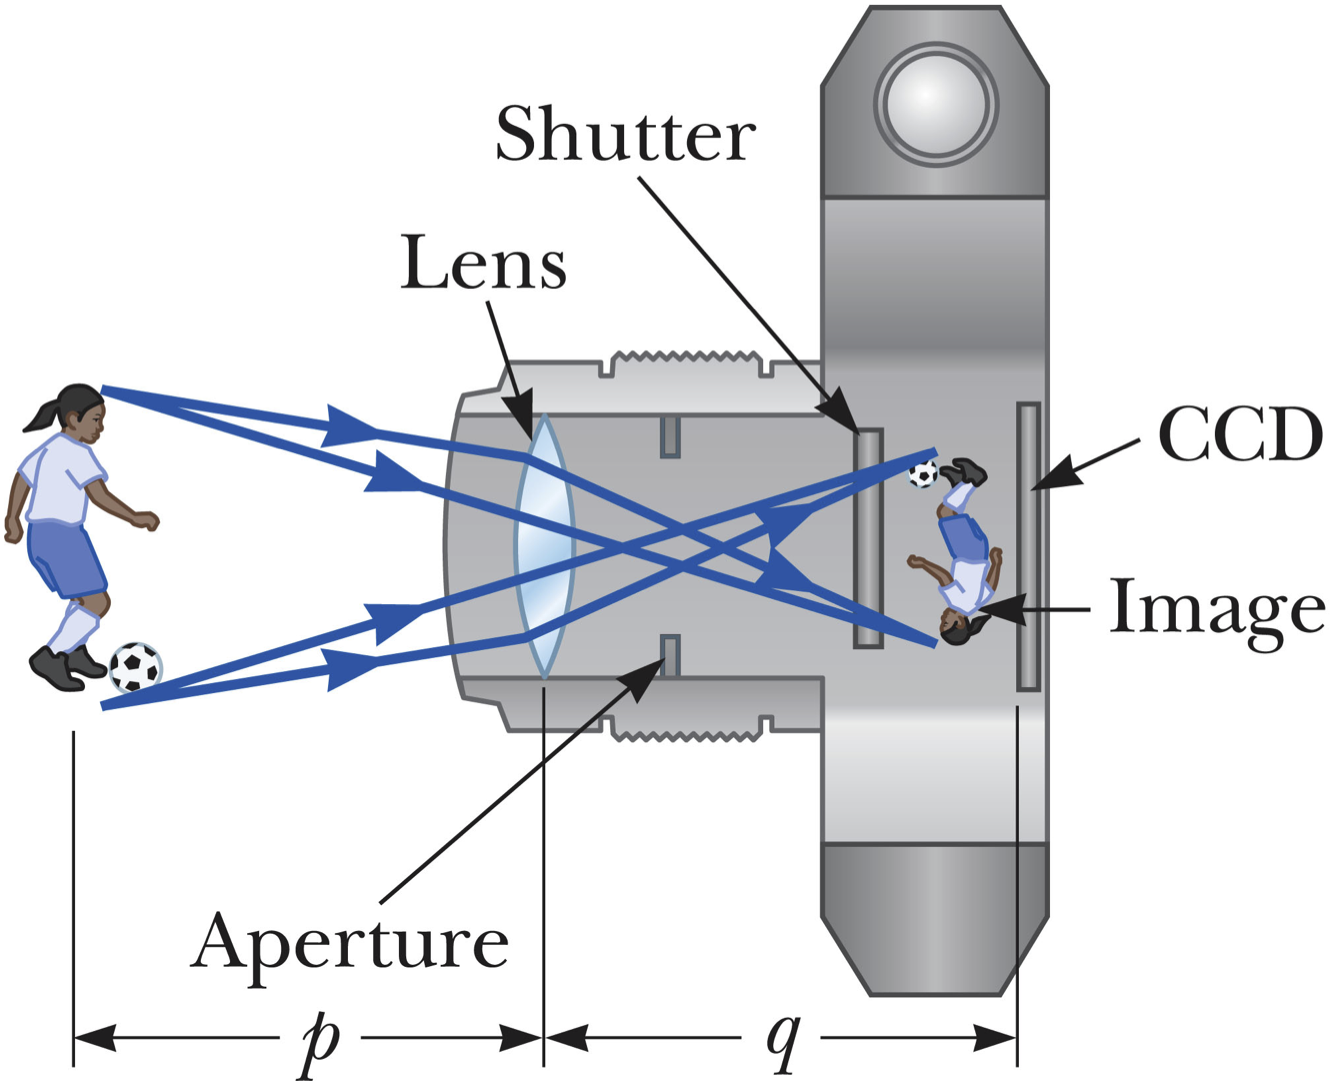
\includegraphics[width=0.5\textwidth]{images/lens_camera}
    \caption{Lens camera. Adapted from \cite{coltonPhysics1232012}} \label{fig:lens_camera}
\end{figure}

However, it is impossible to construct a model which is both simple and exact for the lens cameras, as the behavior of lenses are very complex. As such, it is mathematically convenient to approximate the camera as a pinhole camera. In doing so, we ignore lens distortion, but it distills the behavior of a camera to its most fundamental and essential dynamics: the projection of points in 3D space onto the flat 2D image plane. 

\subsubsection{Pinhole Camera Model}

A pinhole camera is a simple camera without a lens. It instead relies on the use of a tiny hole as the aperture of the camera, and light rays pass through the hole, projecting an inverted image onto the image plane. The pinhole camera model is based on the pinhole camera, however it goes further by making the assumption that the aperture is infinitely small. This means that any incoming light ray would only travel in straight lines, going through the pinhole mapping to one singular point on the image plane. 

\begin{figure}[H]
    \centering
    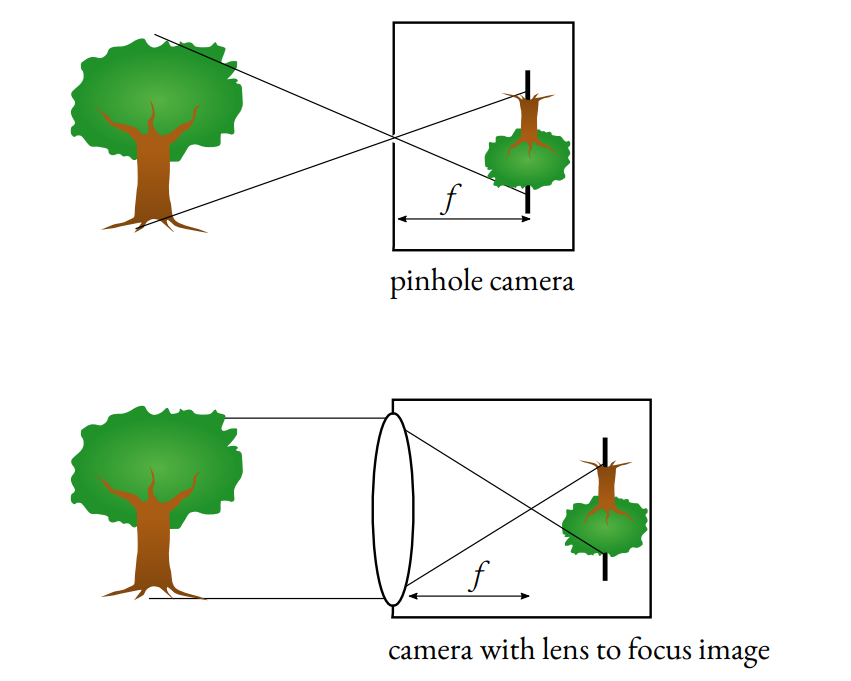
\includegraphics[width=0.7\textwidth]{images/pinhole_vs_lens}
    \caption{Difference between a pinhole camera and a lens camera. Adapted from \cite{leCameraModel2018}}
\end{figure}

If necessary, one could reintroduce distortion and shear terms in order to minimize the error, but this is often not needed for low to medium precision applications, as the distortion of modern lenses are already minimal. The pinhole camera model is a sufficient, and its simplicity has led it to become one of the most frequently employed camera models in the field of camera calibration. 

\subsection{Calibration Object}

The calibration object is an object with known dimensions and features which is often employed in camera calibration to establish a mapping between the 3D world and 2D image space. By capturing images of the calibration object, one can establish correspondences between points in the scene and pixels in the images, which can then be used to deduce the camera's intrinsic and extrinsic parameters. Calibration objects can be constructed in many ways, and they can be separated into different categories based the dimension of the calibration object \footcite{zhangCameraCalibration2007}. 

\begin{itemize}[leftmargin=!, itemindent=-4ex]
    \item \textbf{3D object based calibration} -- Performed by using a calibration object whose geometry is known to very high precision. Typically, the calibration object consists of 2 or 3 orthogonal planes, although a plane whose precise translation is known may also be used, which also yields 3D reference points \footcite{zhangCameraCalibration2007}. Using 3D objects is typically preferred, as it yields the highest accuracy \footcite{zhangCameraCalibration2007}, and the mathematics required is the simplest.
    \item \textbf{2D plane-based calibration} -- The most common technique is known as \emph{Zhang's method}, and it requires a planar object (often a checkerboard pattern), and various pictures of this plane are taken at different orientations \footcite{zhangFlexibleNew2000}. Knowledge of the translation of the plane is not necessary. Due to its easier setup and good accuracy, it is the best choice in most situations. In fact, the most commonly used camera vision programming library, \texttt{OpenCV}, is geared towards this type of calibration. 
    \item \textbf{1D line-based calibration} -- Typically requires analyzing more than three photographs with straight lines which are not parallel with each other \footcite{chuLineBasedCamera2005}. 
\end{itemize}

One can also calibrate cameras without a calibration object, using featuring tracking of objects in the scene to estimate camera parameters. This process is often referred to as self-calibration or auto-calibration. However, this is less preferable, as it involves a lot of estimation of parameters, which means that it becomes a more mathematically complex problem, and may not be able to achieve the level of accuracy of calibration achievable using known calibration patterns \footcite{zhangCameraCalibration2007}. As such, it is typically the only chosen when pre-calibration is impossible. 

For this paper, I will focus on calibration using a 3D calibration object, because the mathematics behind it is simpler, and the techniques used in 3D-based calibration are well-established. By concentrating on 3D-based calibration, this paper aims to leverage the simplicity and reliability of established mathematical methods to gain a better understanding behind the mathematical techniques and strategies employed in camera calibration.
